\documentclass[a4paper,11pt]{article}

\usepackage[utf8]{inputenc}
\usepackage{CJKutf8}

\usepackage[margin=2.3cm]{geometry}
\usepackage{amsmath,amssymb}
\usepackage{booktabs}
\usepackage{graphicx}
\usepackage{hyperref}
\usepackage{xcolor}
\usepackage{fancyvrb}
\usepackage{enumitem}
\usepackage{float}

\hypersetup{
  colorlinks=true,
  linkcolor=blue,
  urlcolor=blue
}

\title{Influence Functions 复现报告 \\ \large Koh \& Liang  Figure 2 中间图}
\author{Zhe Fu}
\date{2026 年 4 月 15 日}

\begin{document}
\begin{CJK*}{UTF8}{gbsn}

\maketitle

\section*{TL;DR}

我在 MNIST 上训了一个带 L2 正则的 logistic regression（n=55000），
按论文方法实现了 influence function 的两种算法（CG 精确解 + LiSSA 随机近似），
然后用 leave-one-out 重训练做了 ground truth 验证，
最后 Pearson = \textbf{0.9983}，Spearman = \textbf{0.9890}，sign match = \textbf{1.0000}，
和论文 Figure 2 中间那张图吻合。

过程中踩了三个坑（LiSSA 有效正则系数算错、CG 迭代步数太少、LOO 的 float32 精度不够），
下面详细说。

\section{我在复现什么}

论文的核心公式：要估计``如果把训练点 $z$ 稍微上调一点点权重，测试点 $z_{\text{test}}$ 的损失会怎么变''。
他们的答案是：
\[
\mathcal{I}_{\text{up,loss}}(z, z_{\text{test}})
  = -\, \nabla_\theta L(z_{\text{test}})^\top \, H_{\hat\theta}^{-1} \, \nabla_\theta L(z)
\]

直接算 $H^{-1}$ 不现实（我这边参数维度 $d = 784 \times 10 = 7840$），所以先算
\[
s_{\text{test}} = H_{\hat\theta}^{-1} \, \nabla_\theta L(z_{\text{test}})
\]
然后对每个训练点只需要一次内积：$-s_{\text{test}} \cdot \nabla L(z)$。
关键就是怎么算出这个 $s_{\text{test}}$。论文给了两种办法，我都实现了。

\textbf{Figure 2 中间图的意思}：x 轴是真实的 LOO 损失差（把某个训练点删掉重训练，测试点损失变了多少），
y 轴是 LiSSA 随机近似预测的损失差。如果两种方法都对，点应该落在 $y=x$ 上。

\section{整体流程}

\begin{Verbatim}[frame=single, fontsize=\small]
train_linear_mnist.py              train baseline
         |
         v
inspect_test_point.py              choose a test point (idx=8, misclassified)
         |
         +------> cg_inverse_hvp.py              (exact solution)
         |              |
         |              v
         |       s_test_cg_idx8.pt
         |              |
         +------> stochastic_inverse_hvp.py      (LiSSA approximation)
                        |
                        v
                 s_test_idx8_r10_t5000.pt
                        |
                        v
              compute_predicted_influence.py   compute prediction for each train point
                        |
                        v
              loo_retrain_topk.py              LOO retraining for ground truth
                        |
                        v
                  Figure 2 middle plot
\end{Verbatim}

\begin{table}[h]
\centering
\small
\begin{tabular}{lp{8.5cm}}
\toprule
脚本 & 作用 \\
\midrule
\texttt{influence\_utils.py} & 共享工具（模型类、HVP、梯度、loss）\\
\texttt{train\_linear\_mnist.py} & 训 baseline 线性分类器 \\
\texttt{hvp\_sanity\_check.py} & 验证 HVP 实现的线性性 \\
\texttt{inspect\_test\_point.py} & 挑一个分类错的测试点 \\
\texttt{cg\_inverse\_hvp.py} & Conjugate Gradient 算 $s_{\text{test}}$（精确）\\
\texttt{stochastic\_inverse\_hvp.py} & LiSSA 算 $s_{\text{test}}$（近似）\\
\texttt{compute\_predicted\_influence.py} & 对所有训练点算预测损失差 \\
\texttt{loo\_retrain\_topk.py} & top-K 留一重训 + 画散点图 \\
\bottomrule
\end{tabular}
\end{table}

\section{踩过的三个坑}

\subsection*{Bug 1：LiSSA 的有效正则系数算错了（核心问题）}

LiSSA 的递推是
\[
h_j = v + (1 - \text{damping}) \, h_{j-1} - \frac{H_z}{\text{scale}} \, h_{j-1}
\]
在期望上收敛到 $(H + \text{damping} \cdot \text{scale} \cdot I)^{-1} v$。
所以 \textbf{真正加进去的额外正则} 是 $\text{damping} \times \text{scale}$，不是 damping 本身。

我一开始用了一些参考实现里的 damping=0.01、scale=50。结果有效正则
$= 0.01 \times 50 = 0.5$，是我真实 L2 正则 0.01 的 \textbf{50 倍}。
这相当于在解一个完全不同的方程，所以随机近似和 CG 的结果严重不一致。

\textbf{修法}：既然 L2=0.01 已经让 Hessian 严格正定了，就不需要额外 damping。
设 damping=0，scale=25（scale 是为了保证 $\|H_z / \text{scale}\| < 1$ 让递推收敛稳定）。

\subsection*{Bug 2：CG 迭代步数太少}

参数维度 7840，一开始设的 \texttt{MAX\_CG\_ITERS=30} 不够。CG 理论上在 $d$ 步内收敛，
实际上因为 L2 让条件数不错，200 步以内就 converge 到 tol=1e-8 了。

\textbf{修法}：\texttt{MAX\_CG\_ITERS} 从 30 改到 200，加上残差提前停止。

\subsection*{Bug 3：LOO 的精度问题（最坑的一个）}

LOO 重训练时要算``删掉一个点后测试损失的变化''，这个差通常在 1e-3 到 1e-5 量级。
原本用 float32 + L-BFGS warm-start，结果很多点的 actual diff 都是精确的 0.0
（散点图上一整条横带贴在 $x=0$）。

原因两个叠加：
\begin{enumerate}[leftmargin=1.3em, itemsep=2pt]
  \item \textbf{float32 精度不够}：warm-start 起点已经离最优解 $\sim 10^{-5}$，
        L-BFGS 内部的二次模型需要的精度在 float32 下直接被 round 到 0，
        line search 的步长变成零，优化器不动。
  \item \textbf{默认 tolerance 太松}：PyTorch L-BFGS 的 \texttt{tolerance\_grad=1e-7} 默认值，
        可是 warm-start 的初始梯度是 $O(1/n) \approx 1.8 \times 10^{-5}$，
        第 0 步就满足停止条件，根本没开始迭代就返回了。
\end{enumerate}

\textbf{修法}：float64 + CPU（MPS 不支持 float64）+ \texttt{tolerance\_grad=0} +
\texttt{tolerance\_change=0} + \texttt{max\_iter=200} + strong Wolfe line search。
改完之后 Pearson 从比较差直接跳到 0.998。

\section{最终结果}

\begin{figure}[H]
\centering
\IfFileExists{loo_scatter_top500_middle_idx8.png}{
  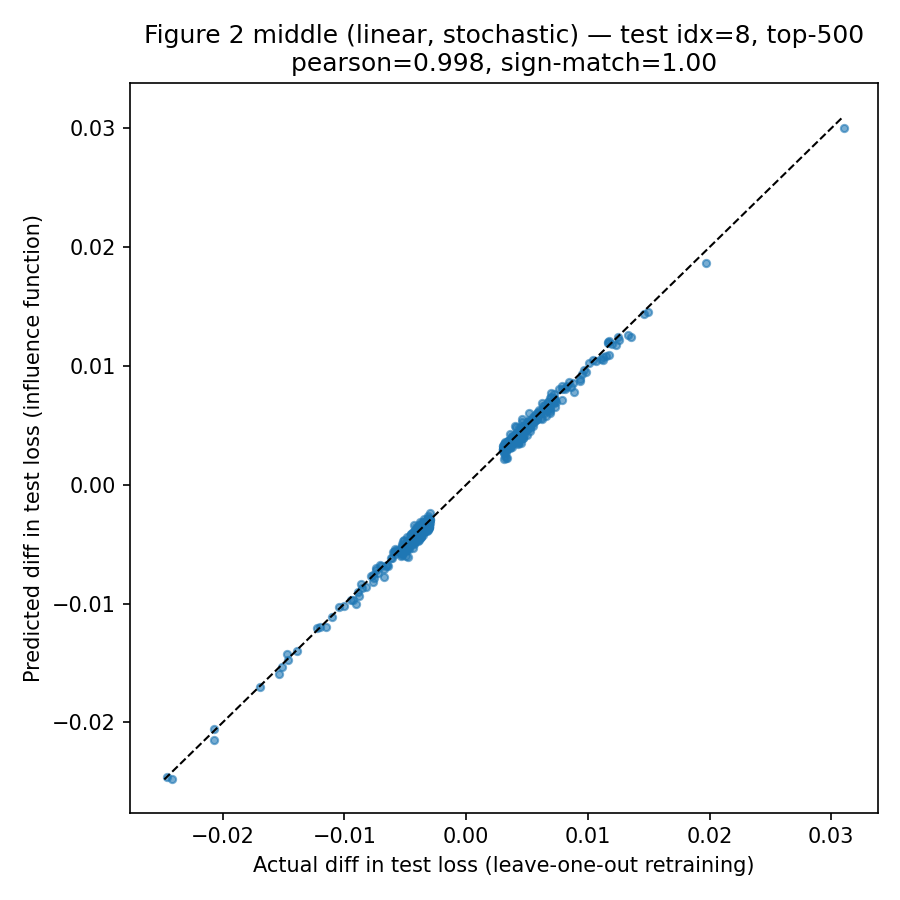
\includegraphics[width=0.65\textwidth]{loo_scatter_top500_middle_idx8.png}
}{
  \fbox{\parbox{0.75\textwidth}{
    \centering
    缺少图片文件：\texttt{loo\_scatter\_top500\_middle\_idx8.png}\\
    请把该图片放到与本 .tex 同一目录。
  }}
}
\caption{Figure 2 中间图复现。x 轴：LOO 真实损失差。y 轴：LiSSA 预测损失差。}
\end{figure}

\begin{table}[h]
\centering
\begin{tabular}{lc}
\toprule
指标 & 值 \\
\midrule
Pearson correlation & 0.9983 \\
Spearman correlation & 0.9890 \\
Same-sign ratio & 1.0000 \\
Top-K & 500（按 CG 的 $|\text{influence}|$ 取）\\
测试点 & idx=8，真实标签 5，模型预测 6 \\
\bottomrule
\end{tabular}
\end{table}

按照论文 Figure 2 中间图的 protocol：用 CG 的 influence 绝对值排序选 top-500，
再把 LiSSA 对这 500 个点的预测放到 y 轴。这样挑点和预测两个步骤分开，
随机噪声不会污染选点。

\section{我搞懂了什么，没搞懂什么}

\textbf{理解到的}：
\begin{itemize}[leftmargin=1.3em, itemsep=2pt]
  \item 为什么要用 HVP 而不是显式组装 Hessian（$d \times d$ 内存爆炸）
  \item Pearlmutter 的 trick（对 $\nabla L \cdot v$ 这个标量再求一次导 = $Hv$，全自动微分）
  \item CG 为什么在正定矩阵上好用，以及 L2 正则在这里实际是起到 preconditioning 的作用
  \item LiSSA 为什么要 scale（让 $\|H_z/\text{scale}\| < 1$ 才是一个收缩映射）
\end{itemize}

\textbf{还不太清楚的}：
\begin{itemize}[leftmargin=1.3em, itemsep=2pt]
  \item 对非凸模型（深网络）Hessian 不正定时 influence function 的行为（论文有讨论但我没深入看）
  \item LiSSA 在高维 + 非凸下的收敛理论保证
  \item 为什么 scale=25 在实践中够用（我用了 MNIST 输入范数的上界估计，
        但更紧的界需要更仔细的分析）
\end{itemize}

\section{下一步想做的}

\begin{itemize}[leftmargin=1.3em, itemsep=2pt]
  \item 在 CNN 上做（对应 Figure 2 右图）
  \item 研究非凸情况下怎么处理负特征值
  \item 看一下 influence function 在数据集清洗 / 错误标注检测上的应用
\end{itemize}

\appendix

\section{关键超参数}

\begin{itemize}[leftmargin=1.3em, itemsep=2pt]
  \item 训练：n=55000，\texttt{L2\_REG=0.01}，L-BFGS 收敛到最优
  \item 测试点：idx=8（一个被分错的 5，模型预测成 6）
  \item CG：\texttt{max\_iter=200}，\texttt{tol=1e-8}
  \item LiSSA：R=10 次重复，T=5000 步，scale=25，damping=0
  \item LOO：top-500，float64，CPU，L-BFGS 零 tolerance，\texttt{max\_iter=200}，warm-start
\end{itemize}

\section{AI 工具使用声明}

我用 Claude 帮忙：
\begin{itemize}[leftmargin=1.3em, itemsep=2pt]
  \item 定位上面说的三个 bug（尤其是 LiSSA 有效正则那个，靠算 fixed point 推出来的）
  \item 检查我写的 HVP 实现对不对（用线性性做 sanity check）
  \item Debug LOO 里 float32 精度问题（从现象反推出 tolerance 阻塞）
  \item 帮助我理解论文中部分公式内容，整理思路
  \item 提供代码思路
\end{itemize}

论文理解、代码架构决策、结果分析、这份报告是我自己写的。

\end{CJK*}
\end{document}
